\chapter{Determination of \lambdaWZ through VBS WH production}
\begin{aquote}{Peter Higgs, Edinburgh University press conference, 2012}
    It's very nice to be right sometimes.
\end{aquote}

\section{Looking for a sign}
Before this work was published, the CMS Collaboration had constrained the \textit{magnitudes} of the HWW (\kW) and HZZ (\kZ) couplings to $|\kW| = 1.02^{+0.11}_{-0.10}$ and $|\kZ| = 1.04^{+0.07}_{-0.07}$, showing precise agreement with the SM values~\cite{NatureHiggsCMS2022}. 
The \textit{sign} of either coupling, however, had not yet been well-determined. 
The relative sign between \kW and \kZ, which is of particular interest, can be expressed more compactly as the ratio between the two couplings:
\begin{equation}
    \lambdaWZ = \frac{\kW}{\kZ}.
\end{equation}
The Standard Model requires $\lambdaWZ = 1$ in order to preserve the ``custodial'' symmetry. 
Meanwhile, certain BSM theories require \lambdaWZ to be negative~\cite{Theory1LambdaWZ}. 
Therefore, in the absence of a significant experimental measurement of the sign of \lambdaWZ, a crucial element of the SM had not been confirmed, and a potential indication of BSM was left unexplored. 

\section{The signal}
The precise determinations of the magnitude of \kW and \kZ~\cite{NatureHiggsCMS2022} were performed by studying processes that are predominantly quadratic in \kV---that is, \kW or \kZ enter the Feynman diagram twice. % add a feynman diagram?
While there were some with a linear dependence, they did not give a strong exclusion of opposite-sign scenarios~\cite{BestCMSLambdaWZ}---in fact they slightly preferred the $\lambdaWZ < 0$ scenario. 
A promising channel to directly probe \lambdaWZ at the LHC is the production of \VH via vector-boson scattering (VBS)~\cite{Theory2LambdaWZ}.
Such a channel is sensitive to the relative sign of \kW and \kZ since the since the cross section $\sigma$ has an interference term that is linear in both \kW and \kZ~\cite{Theory2LambdaWZ}: 
\begin{equation}\label{eq:matrix_elem}
    \sigma \propto |\mathcal{M}|^2 = \kW^2|\mathcal{M}_W|^2 + \kW\kZ\mathcal{M}_{WZ}^2 + \kZ^2|\mathcal{M}_Z|^2
\end{equation}
where the matrix elements for the contributions from the HWW couplings, HZZ couplings, and interference term are denoted as $\mathcal{M}_W$, $\mathcal{M}_W$, and $\mathcal{M}_{WZ}$, respectively. 
Therefore, this channel provides the opportunity to determine the sign of \lambdaWZ with certainty. 
\begin{figure}[htb]
    \centering
    \subfloat{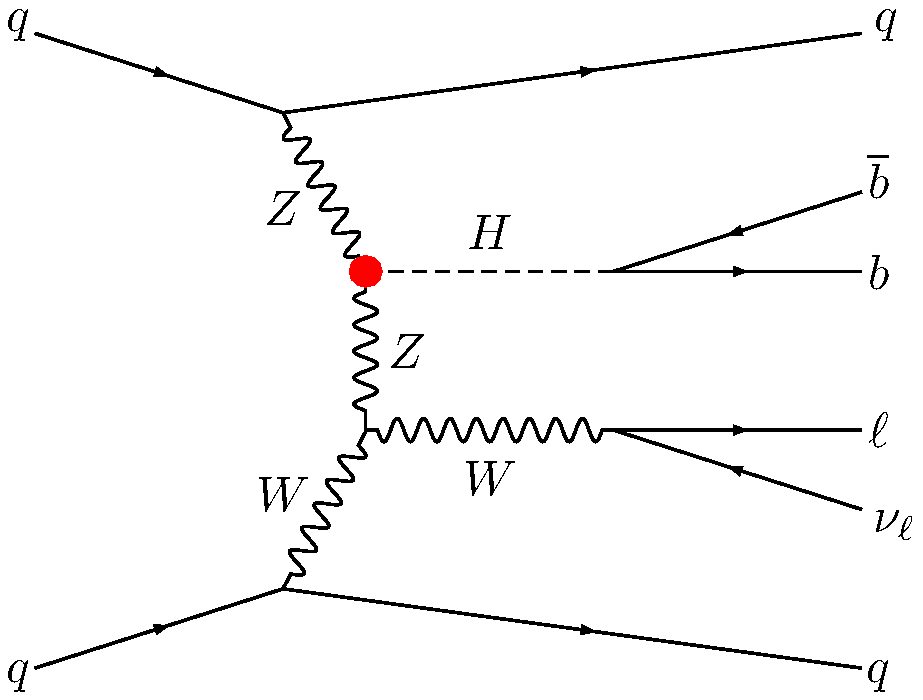
\includegraphics[width=0.3\textwidth]{fig/feynman/vbswh/vbswh_1.pdf}}\quad
    \subfloat{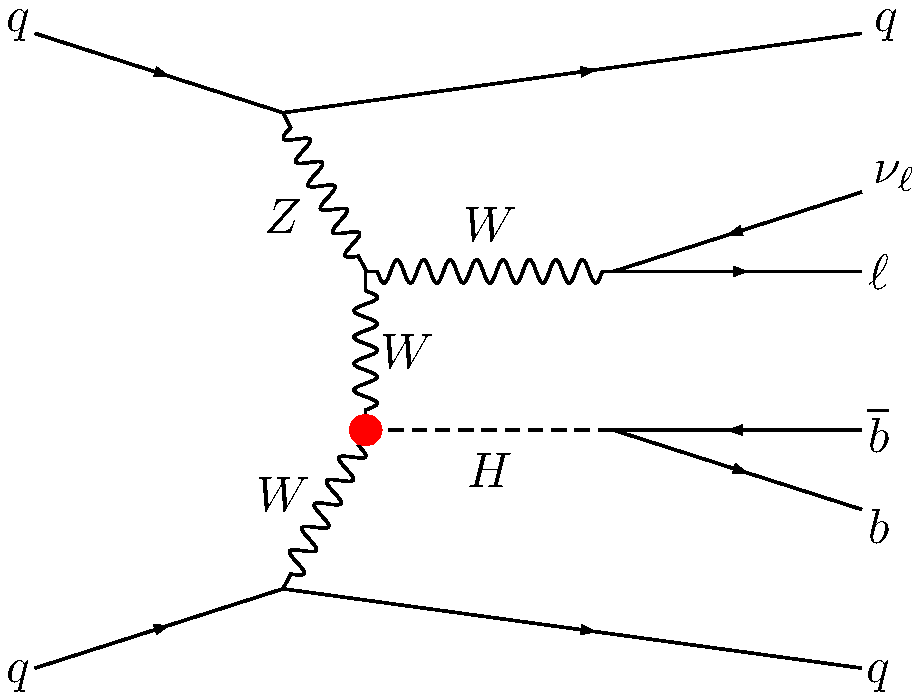
\includegraphics[width=0.3\textwidth]{fig/feynman/vbswh/vbswh_2.pdf}}\quad
    \subfloat{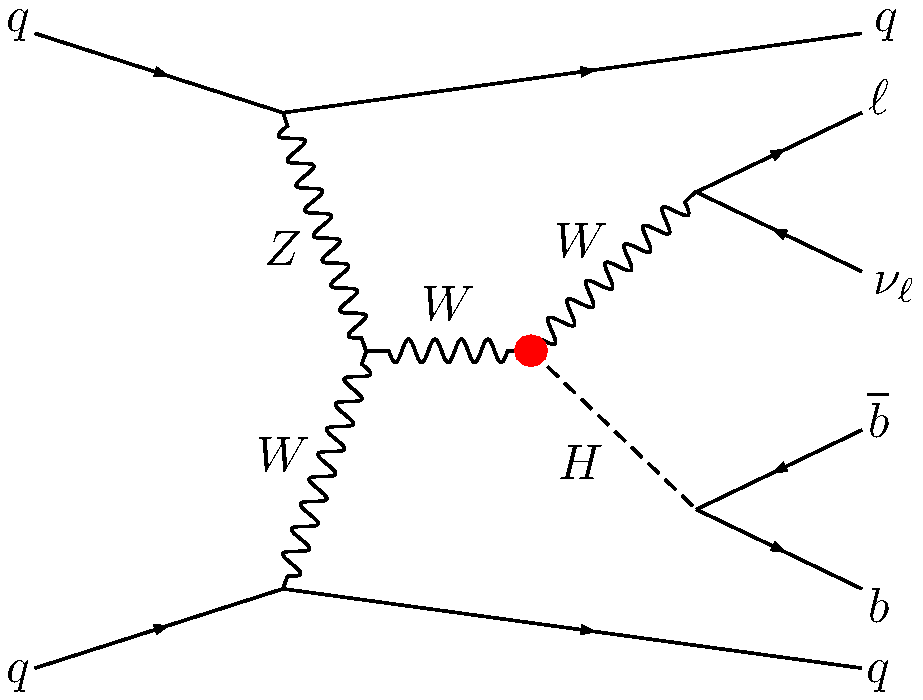
\includegraphics[width=0.3\textwidth]{fig/feynman/vbswh/vbswh_3.pdf}}
    \caption{
        Leading-order Feynman diagrams for VBS production of a W and Higgs boson, where the W decays leptonically and the Higgs decays to b quarks. 
        The Higgs coupling to W bosons \kW and Z bosons \kZ is denoted by a red circle (\textcolor{red}{\ding{108}}). 
    }
    \label{fig:vbswh_feynman}
\end{figure}

\subsection{Signal characteristics}
A specific final state is intentionally selected for its uniqueness---making the signal easier to find amidst the haystack. 
First, leptons are preferred in the final state over jets, due to the sheer size of the ``QCD'' background, the most populous physics process produced at the LHC. 
Then, $\PW\to\ell\nu$ is preferred over $\PZ\to\ell\ell$, since there are fewer backgrounds with only one lepton in the final state. 
Finally, $\PH\to\PQb\PAQb$ has the largest branching ratio, and it can be identified using the latest advances in artificial intelligence. 

While there are a few background processes can produce the target final state, the Monte Carlo (MC) simulation of the signal reveals additional boons. 
The final state particles receive a significant boost for negative \lambdaWZ scenarios (Fig.~\ref{fig:vbswh_lhe}). 
In our preferred final state, this will give a lepton with large \pt, some additional \MET from the neutrino, and two overlapping b-jets reconstructed as a single merged jet. 
Additionally, the cross section of the signal process increases quadratically as \kW or \kZ deviate from the SM value (Fig.~\ref{fig:vbswh_xsecs}). 

\begin{figure}[htb]
    \centering
    \subfloat{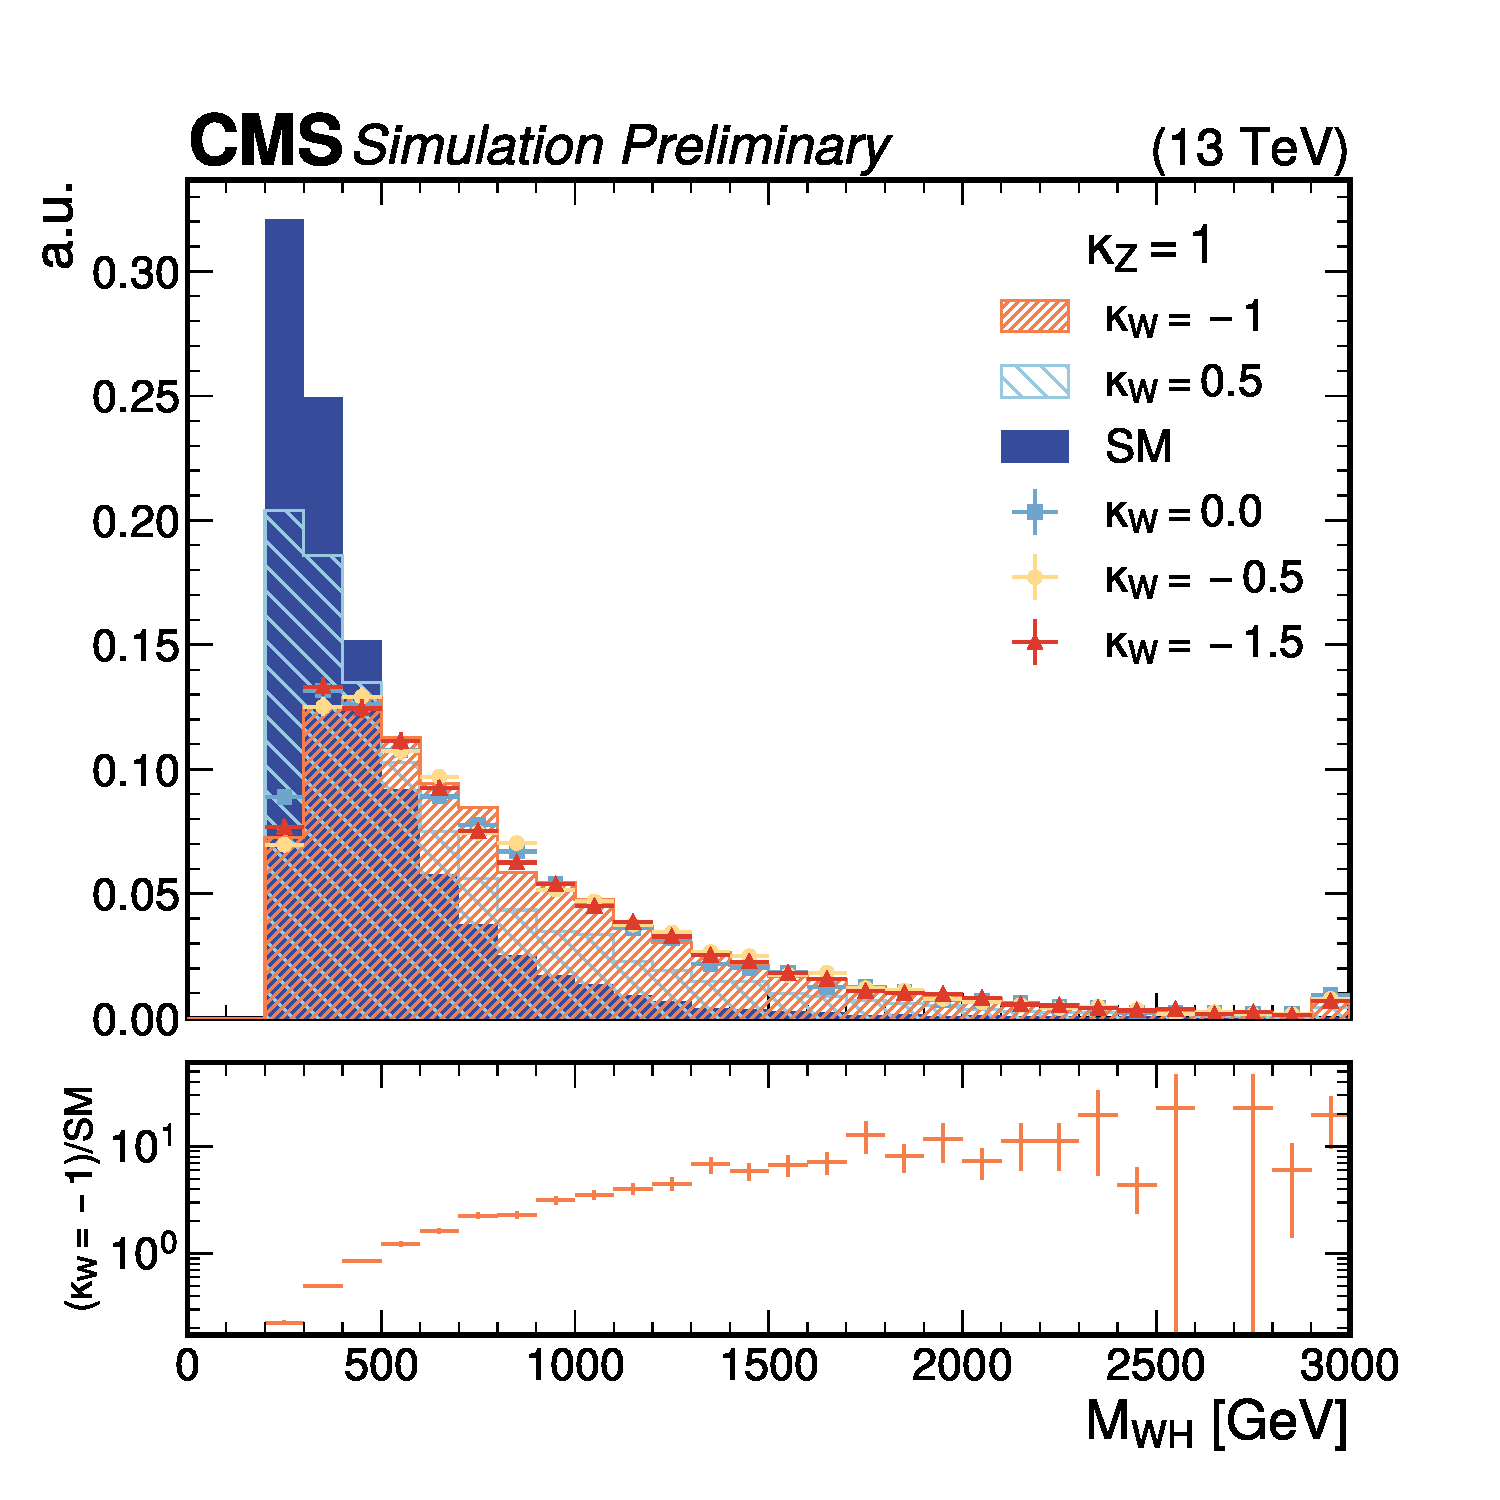
\includegraphics[width=0.45\textwidth]{fig/vbswh/lhe_M_WH_1p0kZ_kWpoints_norm.pdf}\label{fig:lheMWH_kWpoints}}\qquad
    \subfloat{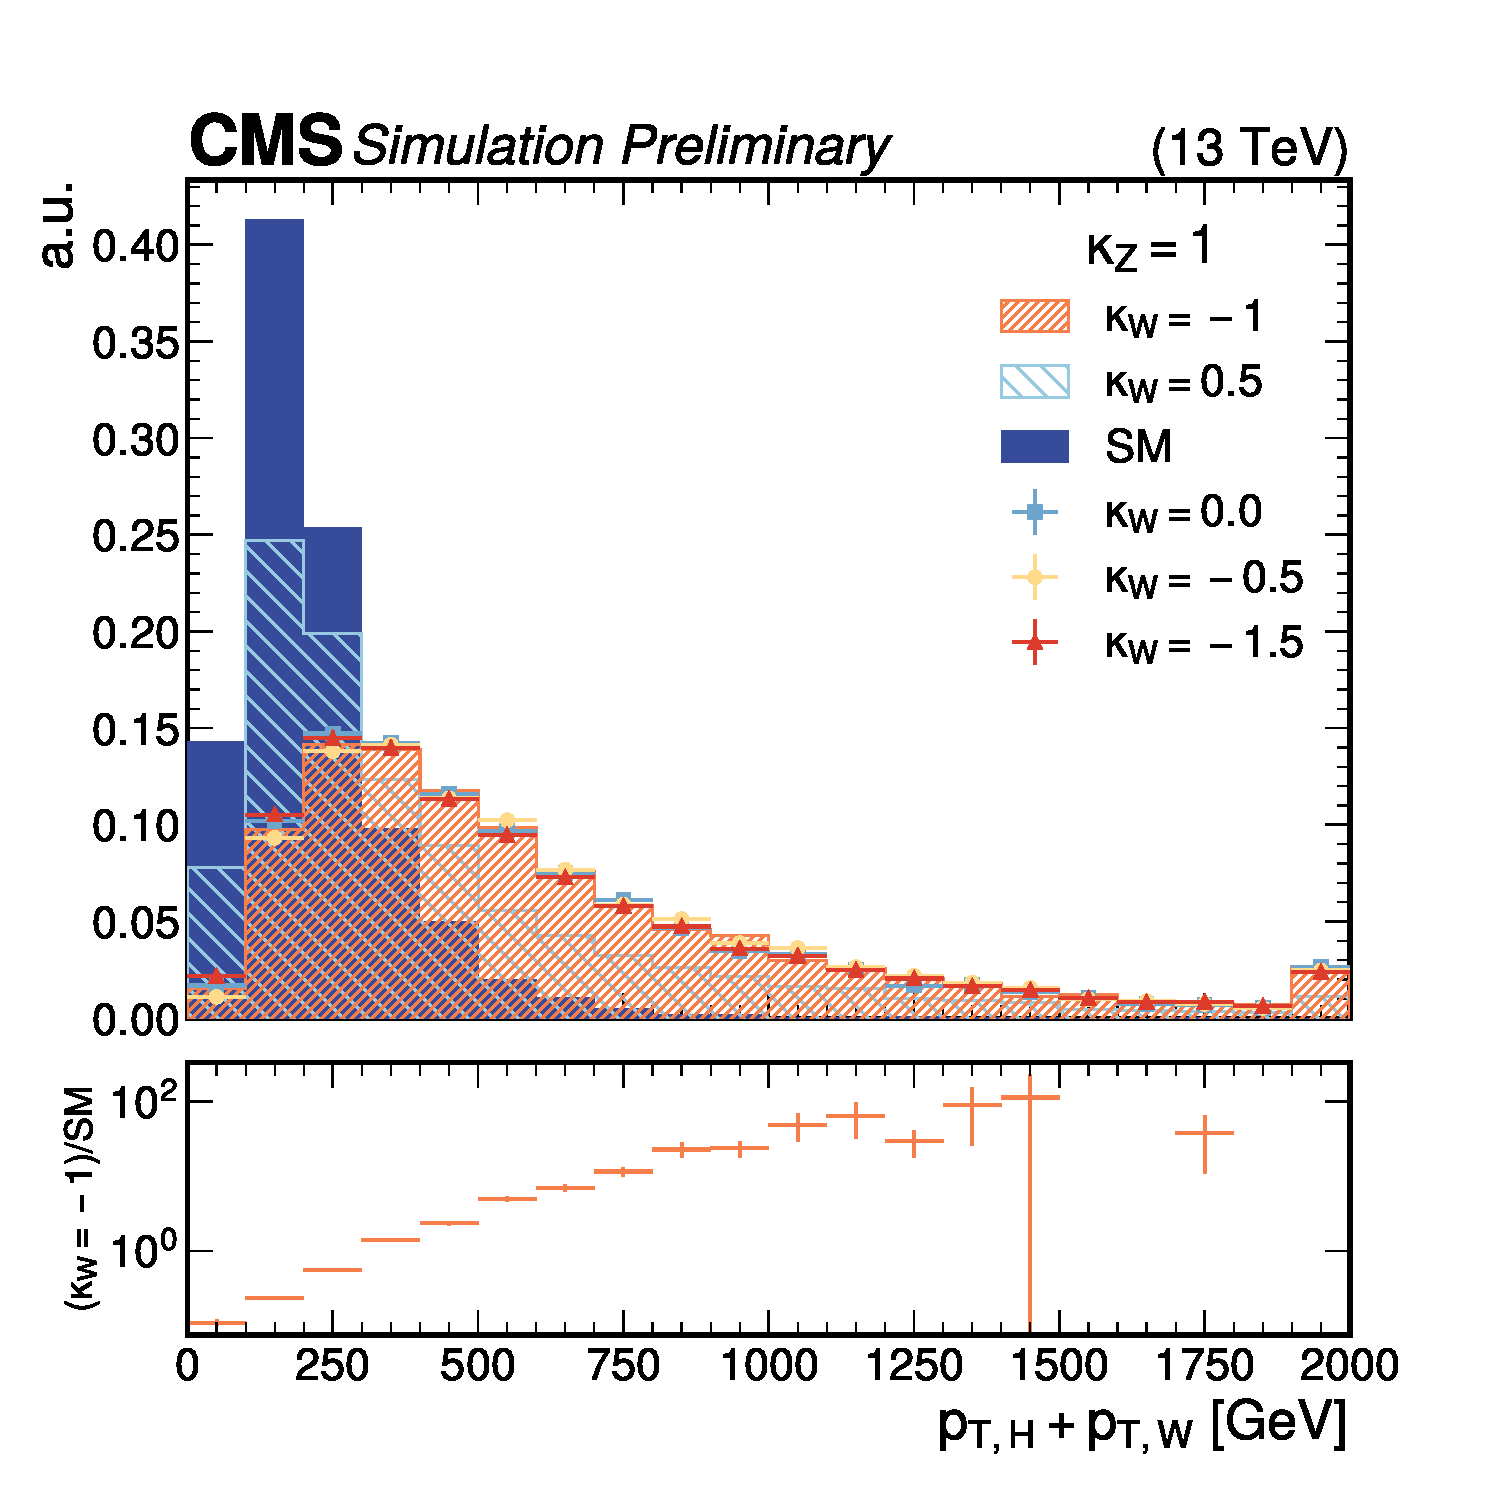
\includegraphics[width=0.45\textwidth]{fig/vbswh/lhe_ST_1p0kZ_kWpoints_norm.pdf}\label{fig:lheST_kWpoints}}\\
    \subfloat{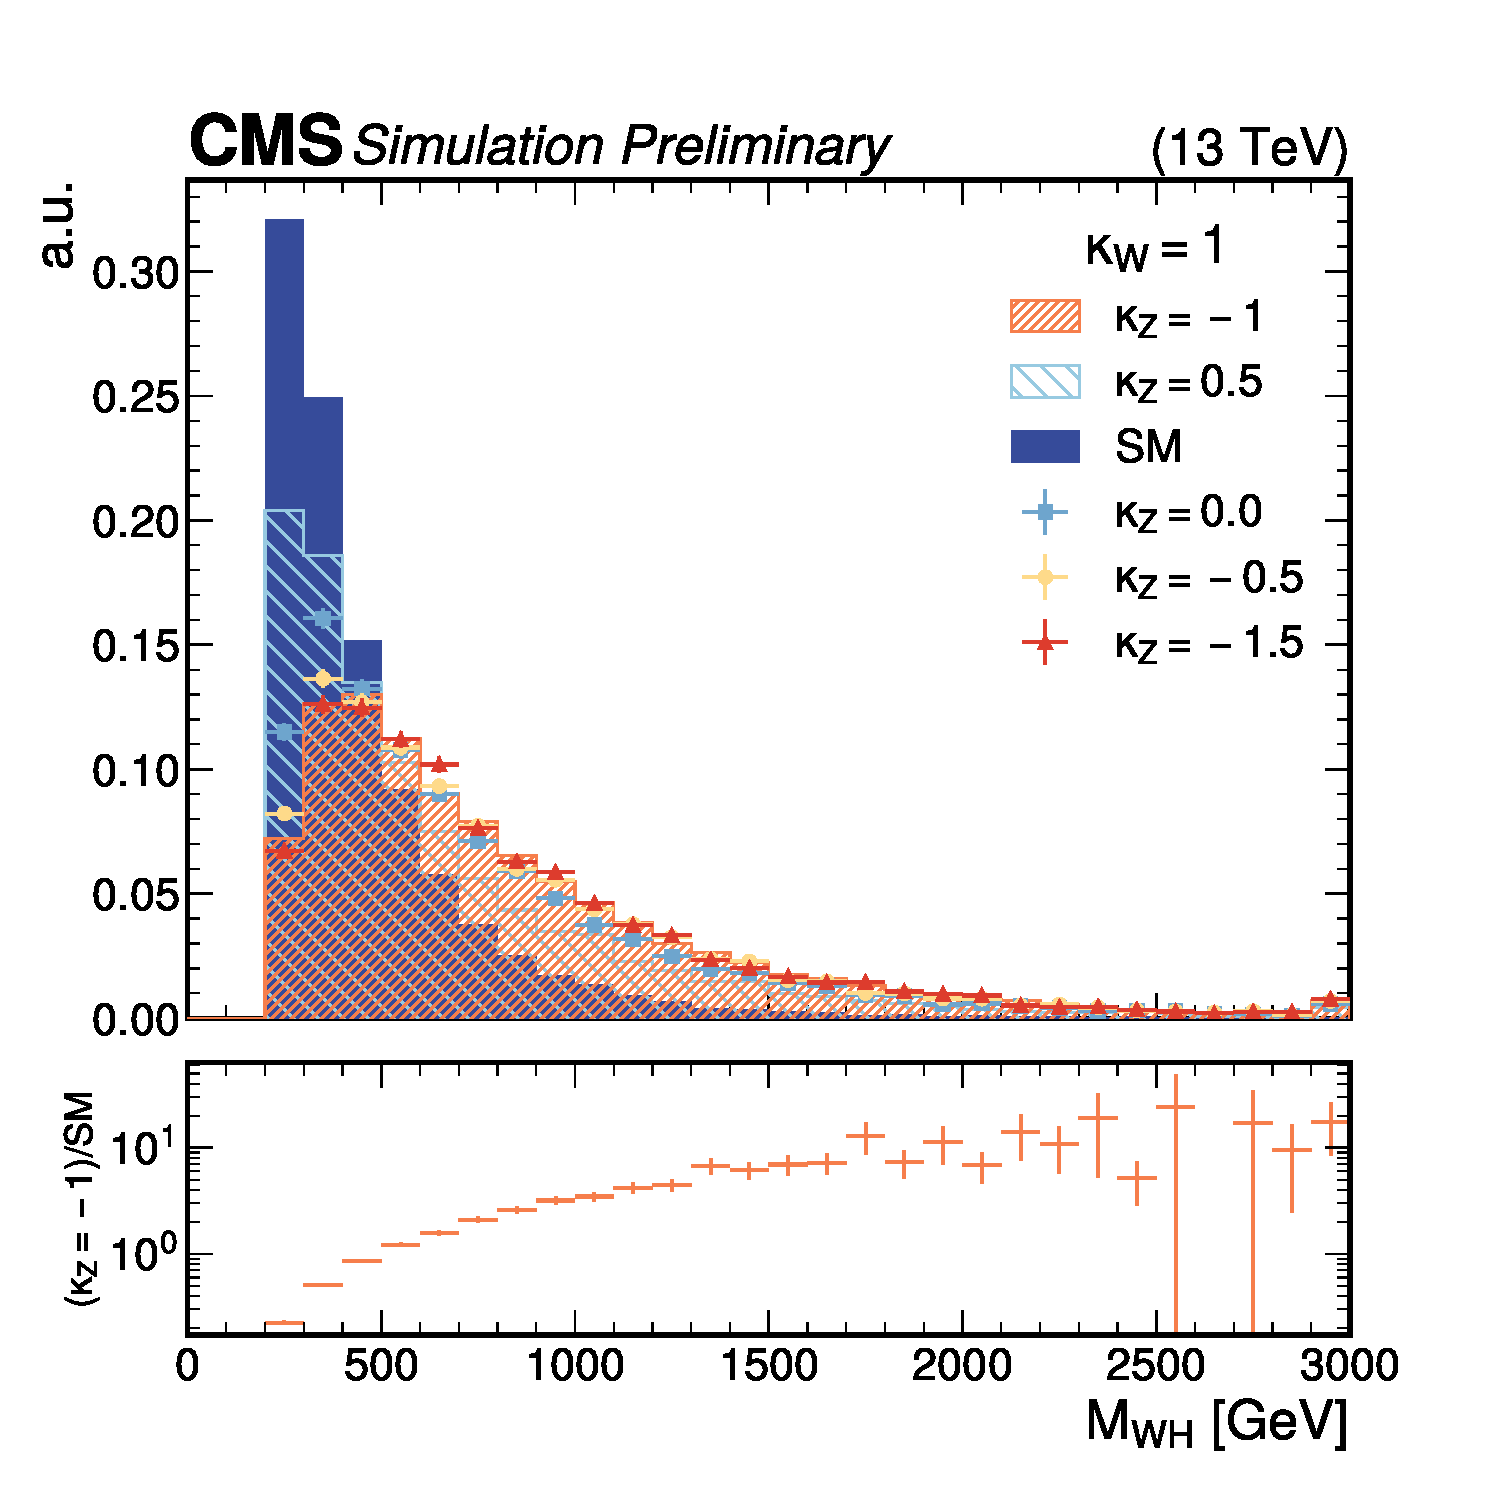
\includegraphics[width=0.45\textwidth]{fig/vbswh/lhe_M_WH_1p0kW_kZpoints_norm.pdf}\label{fig:lheMWH_kZpoints}}\qquad
    \subfloat{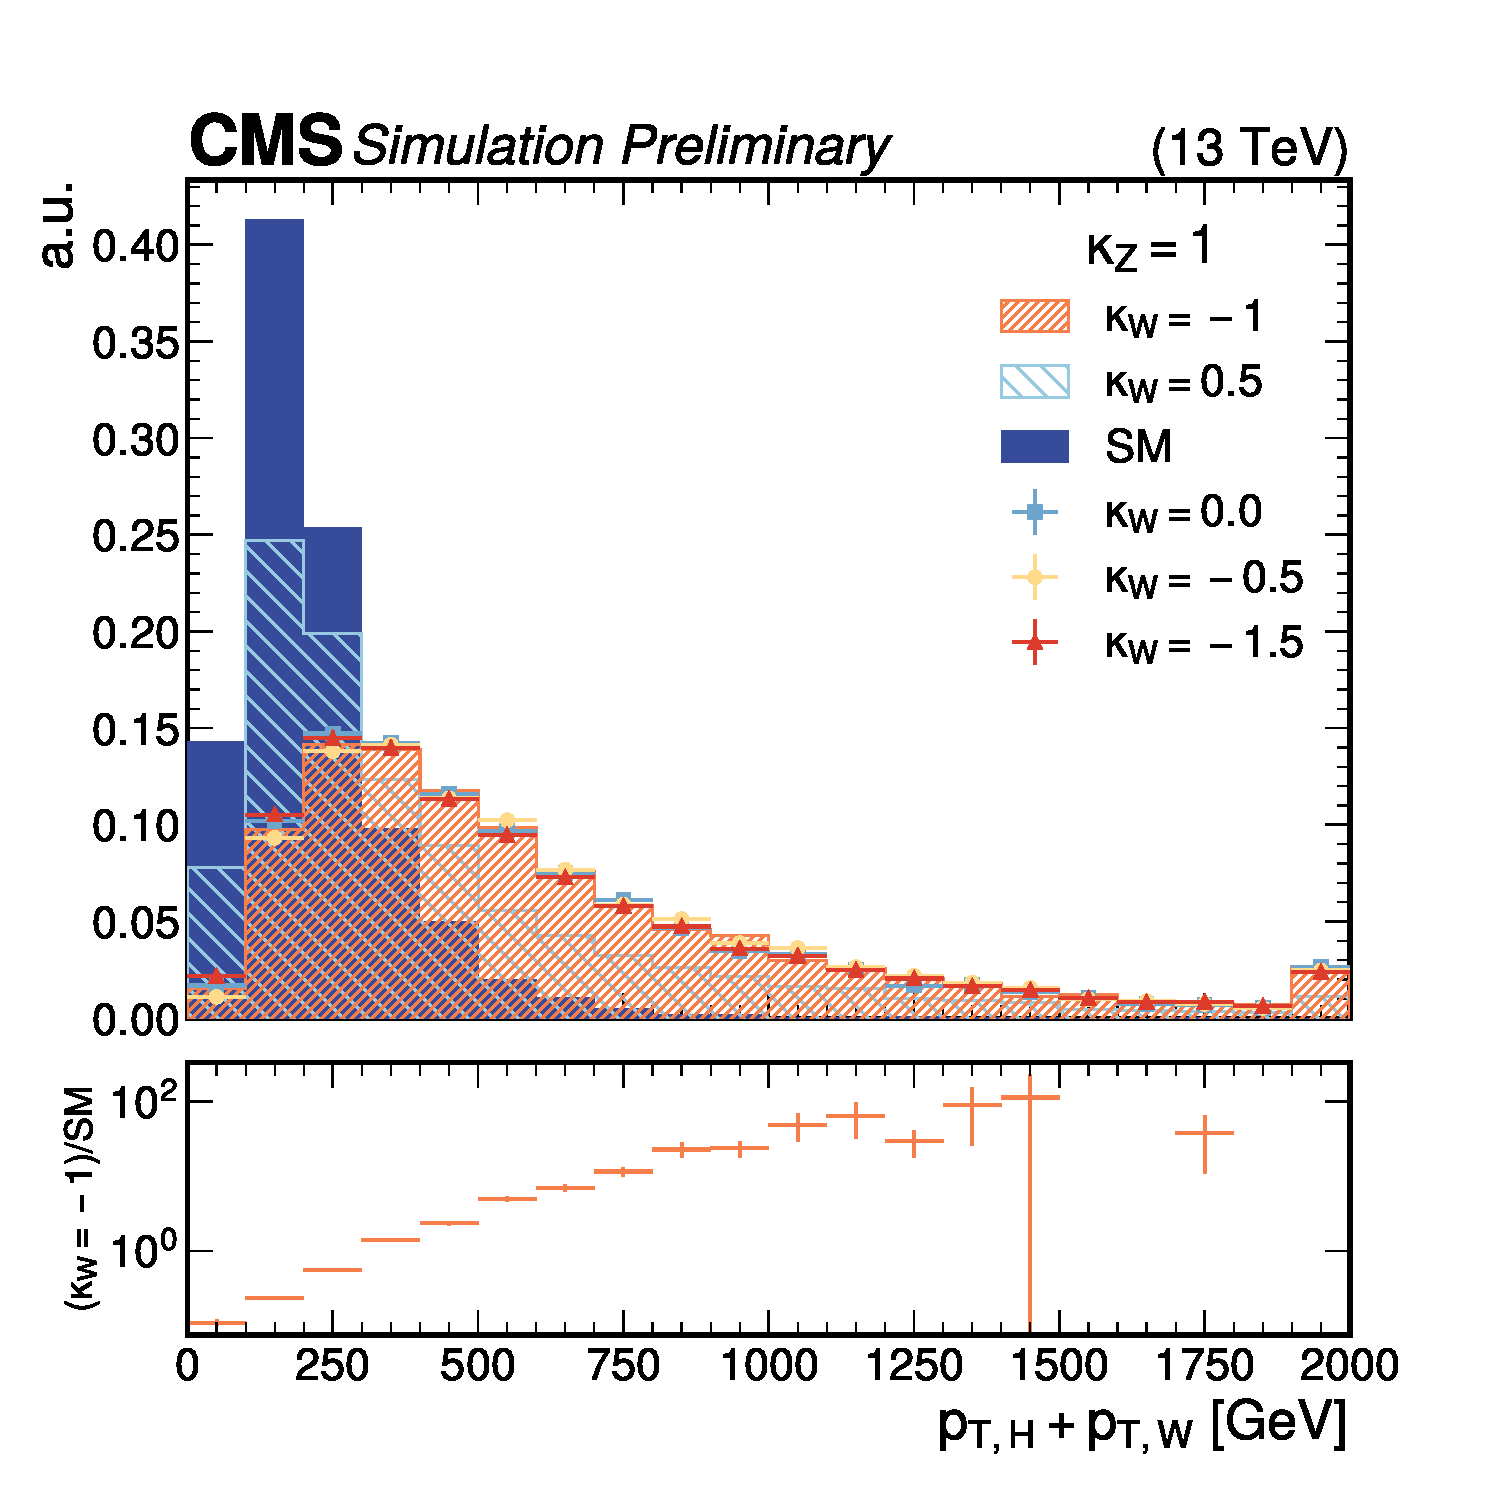
\includegraphics[width=0.45\textwidth]{fig/vbswh/lhe_ST_1p0kZ_kWpoints_norm.pdf}\label{fig:lheST_kZpoints}}
    \caption{
        Histograms of the invariant mass of the \WH system (left) and \ST (right) plotted from \VBSWH Monte Carlo simulation for $\kZ = +1$ (top) and $\kW = +1$ (bottom). 
        All four histograms demonstrate the enhancement in high-energy kinematics due to modifications to \lambdaWZ. 
    }
    \label{fig:vbswh_lhe}
\end{figure}

\begin{figure}[htb]
    \centering
    \subfloat{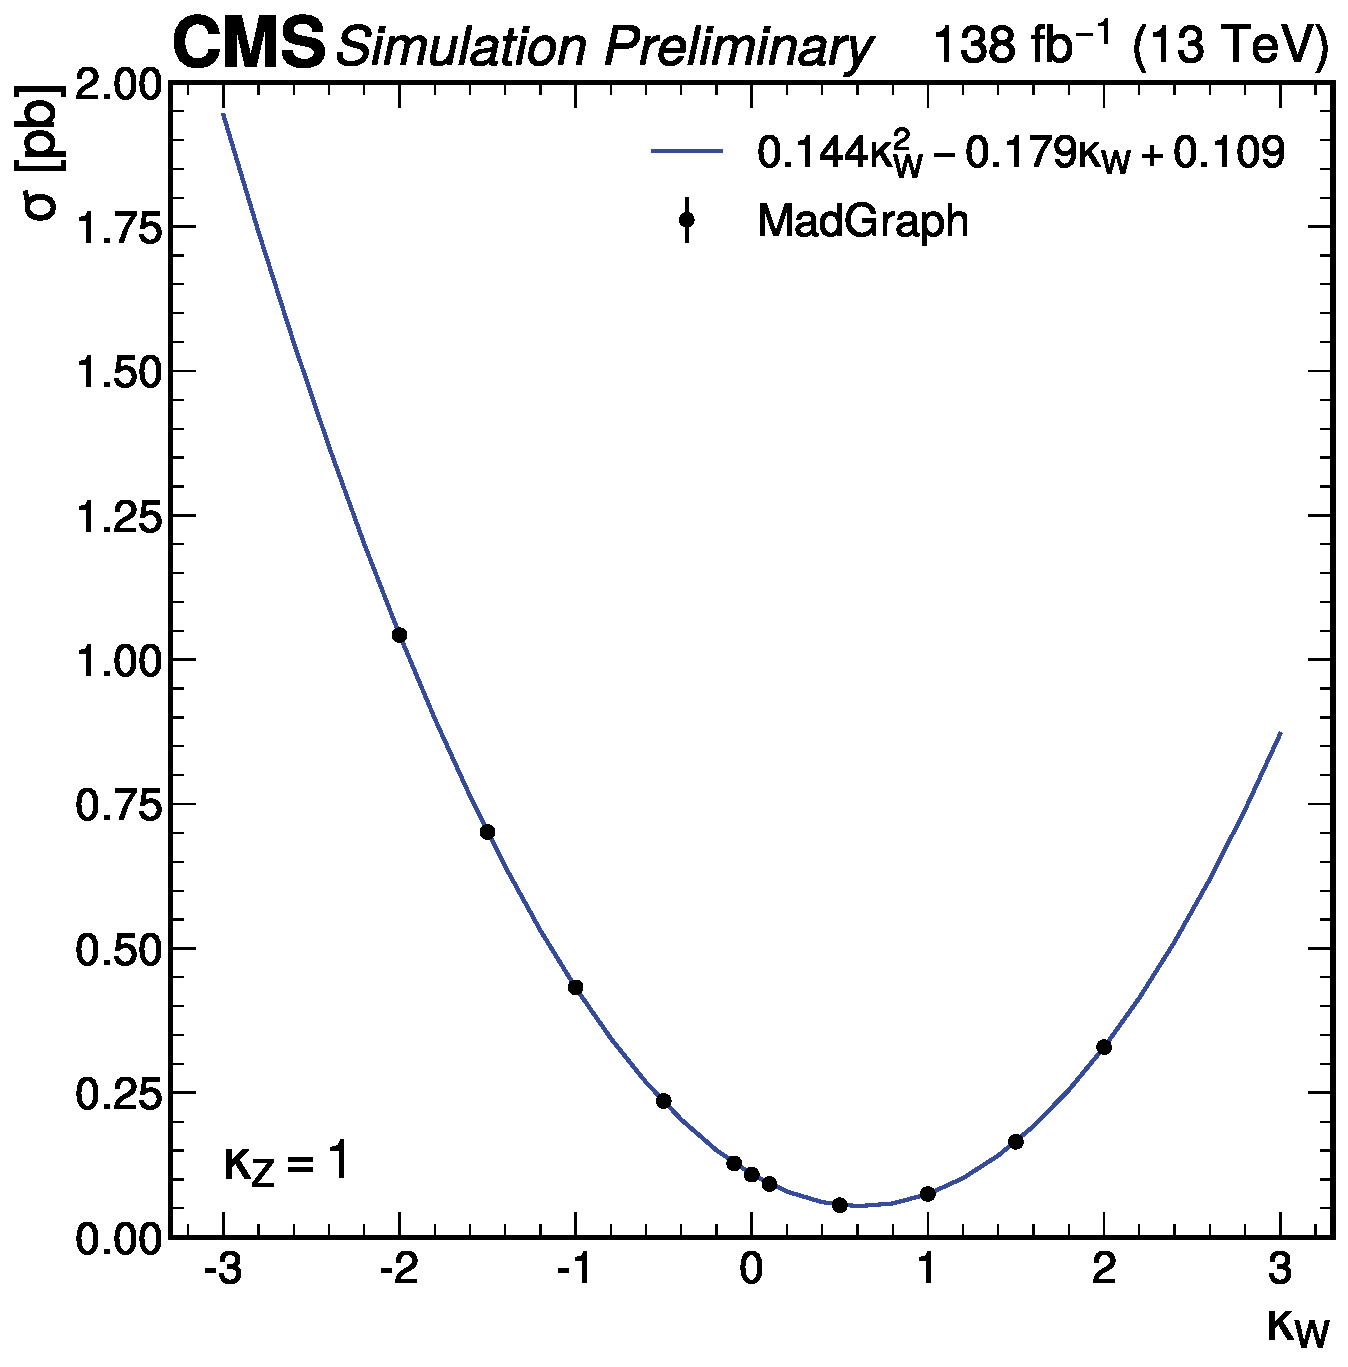
\includegraphics[width=0.45\textwidth]{fig/vbswh/kW_xsecs.pdf}}\qquad
    \subfloat{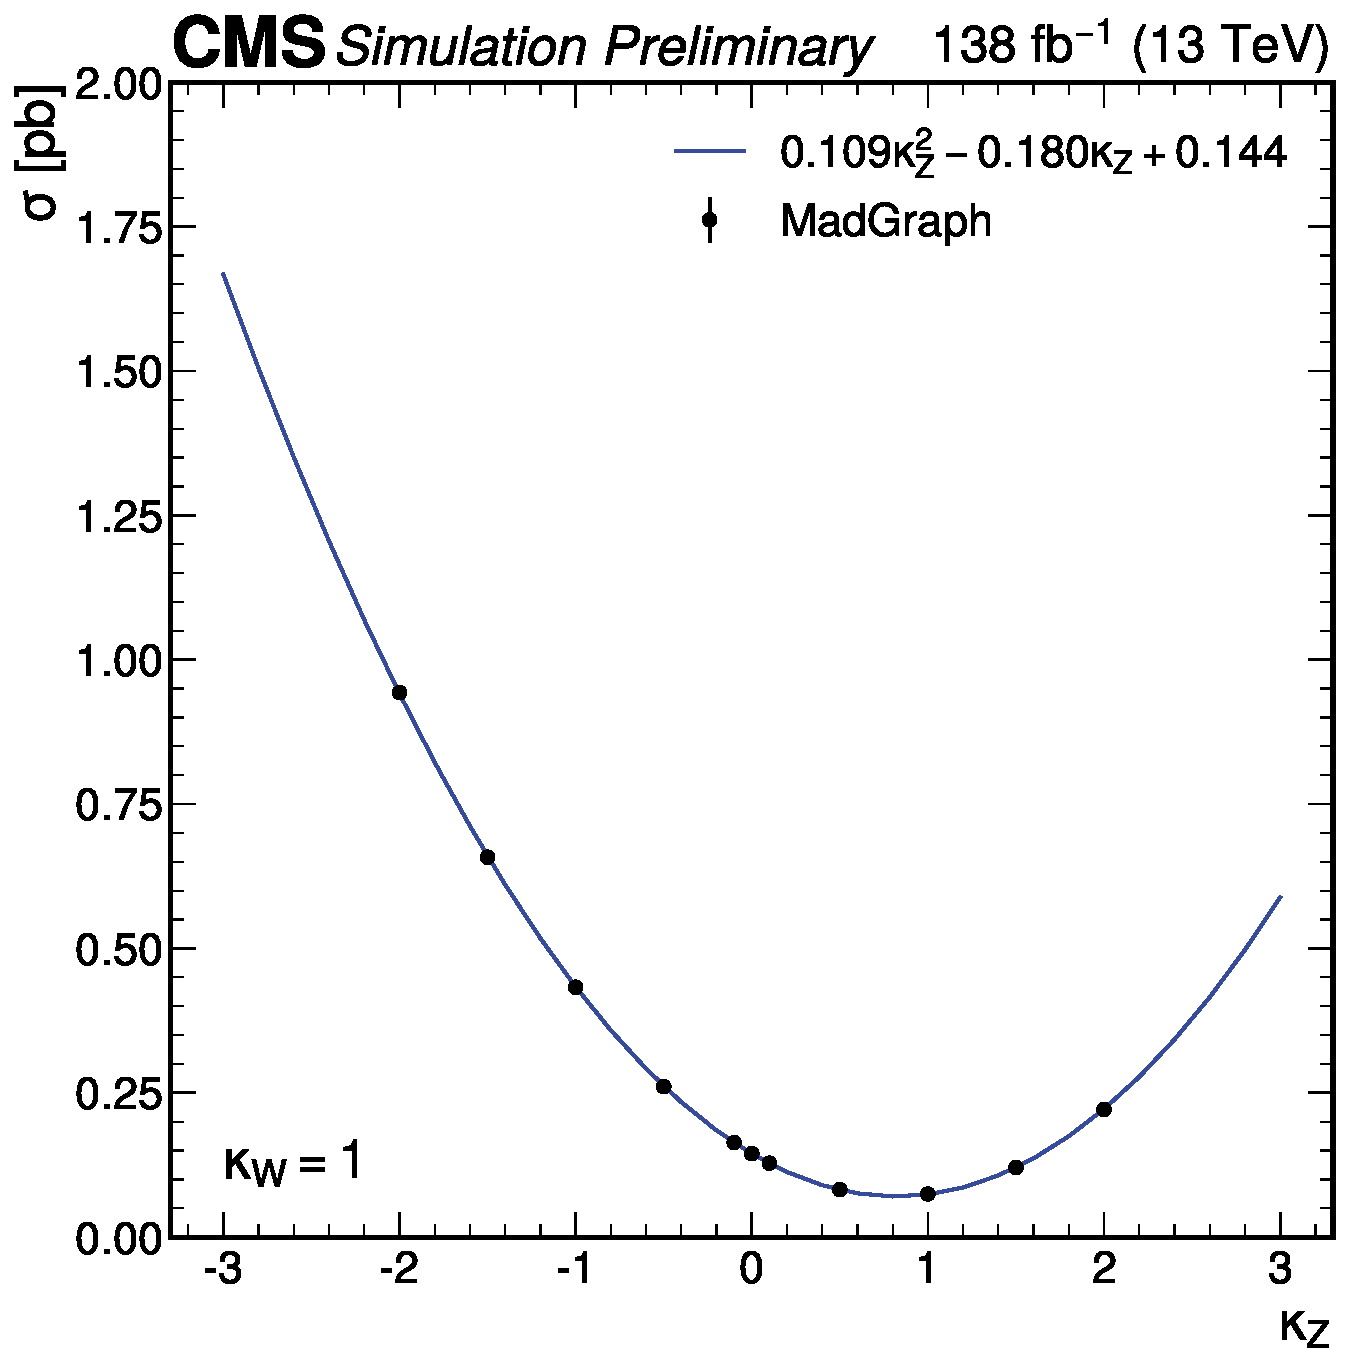
\includegraphics[width=0.45\textwidth]{fig/vbswh/kZ_xsecs.pdf}}
    \caption{
        Plot of the signal cross section as a function of enhancements to \kW (keeping $\kZ = +1$) on the left and to \kZ (keeping $\kW = +1$) on the right. 
        The black points are taken from \MGvATNLO, and the blue curve is the best fit of a 2nd order polynomial to those points. 
        The errors are also plotted, but are smaller than the width of the black points. 
        Importantly, the cross section for $\kW = -1$, $\kZ = +1$ and $\kW = +1$, $\kZ = -1$ are exactly the same. 
    }
    \label{fig:vbswh_xsecs}
\end{figure}

\section{The backgrounds}
In general, background processes for this analysis need a fake\footnotemark{} $\Htobb$ merged jet, two fake\footnotemark[\value{footnote}] VBS jets, one lepton, and some \MET. 
\footnotetext{
    In principle, a background process could have a \textit{real} Higgs boson with large \pt decay to \bbbar or two \textit{real} VBS jets, however SM processes with these kinds of signatures are so rare that they do not represent a significant background for this analysis---in fact, SM VBS WH is one such insignificant background.
}
The main background process for this analysis comes from \ttbar production (Fig.~\ref{fig:ttbar}), wherein a top and antitop quark are produced and both decay to a bottom quark and \PW boson. 
One of the \PW bosons can decay to a real lepton and neutrino, then the fake VBS jets and $\Htobb$ merged jet can come from some combination of the \PQb quarks, quarks from one of the \PW bosons decaying hadronically, and possibly an extra gluon radiated by one of the incoming quarks (Fig.~\ref{fig:ttbar1l}). 
One of the incoming quarks can radiate a \PW or \PZ boson (Fig.~\ref{fig:ttV1l}), which presents additional opportunities for trickery. 
Additional backgrounds come from single-top production, where only one top quark is produced, which then decays to a bottom quark and \PW boson (Fig.~\ref{fig:single_t}). 

\begin{figure}[htb]
    \centering
    \subfloat[$\ttbar + \text{jet}$]{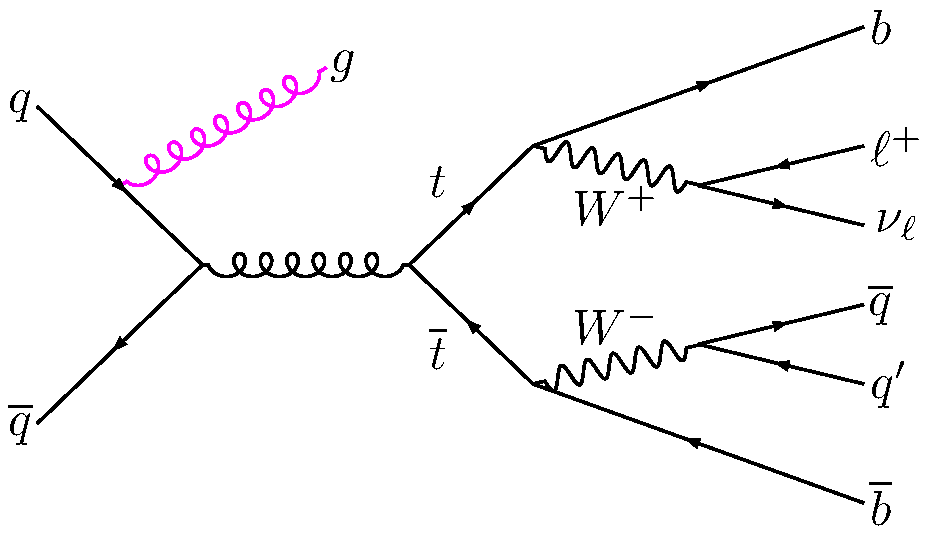
\includegraphics[width=0.4\textwidth]{fig/feynman/ttbar/ttbar_onelep_extraJet.pdf}\label{fig:ttbar1l}}\quad
    \subfloat[$\ttbar + \PV$]{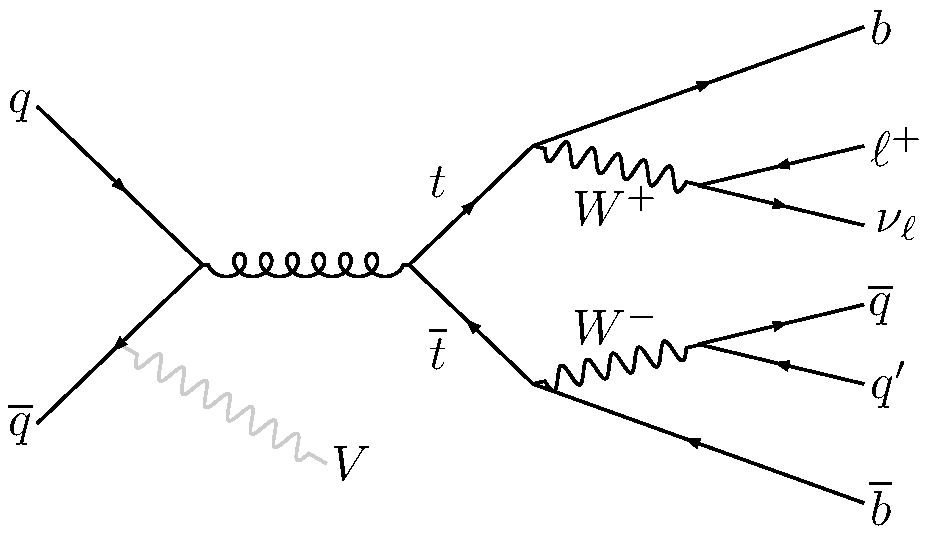
\includegraphics[width=0.4\textwidth]{fig/feynman/ttbar/ttV_onelep.pdf}\label{fig:ttV1l}}
    \caption{
        Feynman diagram for \ttbar production in the single-lepton final state with (a) an extra jet from a gluon or (b) an extra vector boson ($\PV = \PW$ or \PZ) radiated from one of the incoming partons.  
    }
    \label{fig:ttbar}
\end{figure}

\begin{figure}[htb]
    \centering
    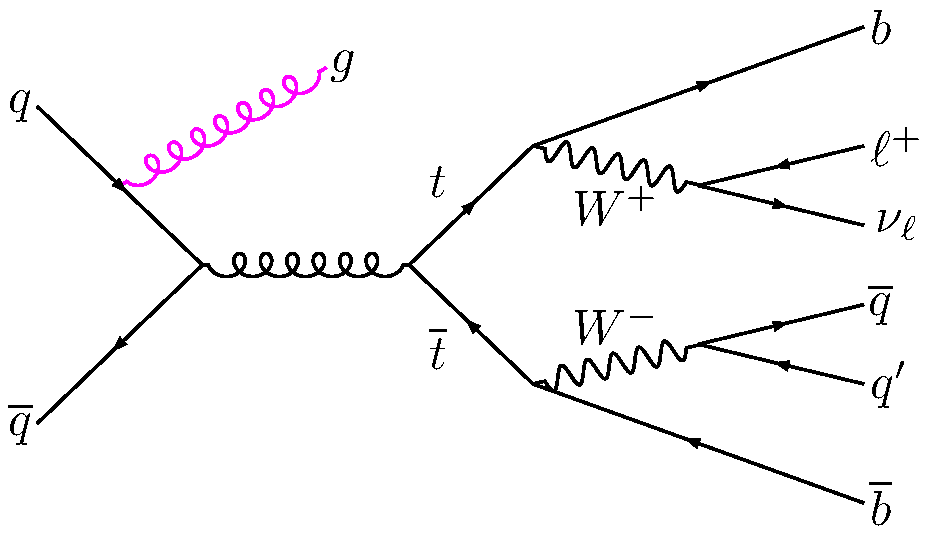
\includegraphics[width=0.4\textwidth]{fig/feynman/ttbar/ttbar_onelep_extraJet.pdf} % FIXME: missing!!
    % \subfloat[$\ttbar + \text{jet}$]{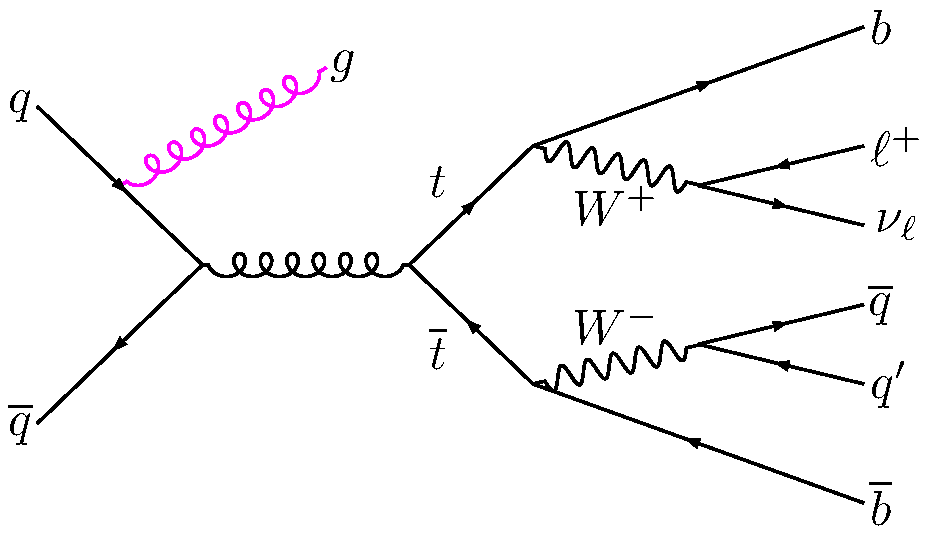
\includegraphics[width=0.4\textwidth]{fig/feynman/ttbar/ttbar_onelep_extraJet.pdf}\label{fig:ttbar1l}}\quad
    % \subfloat[$\ttbar + \PV$]{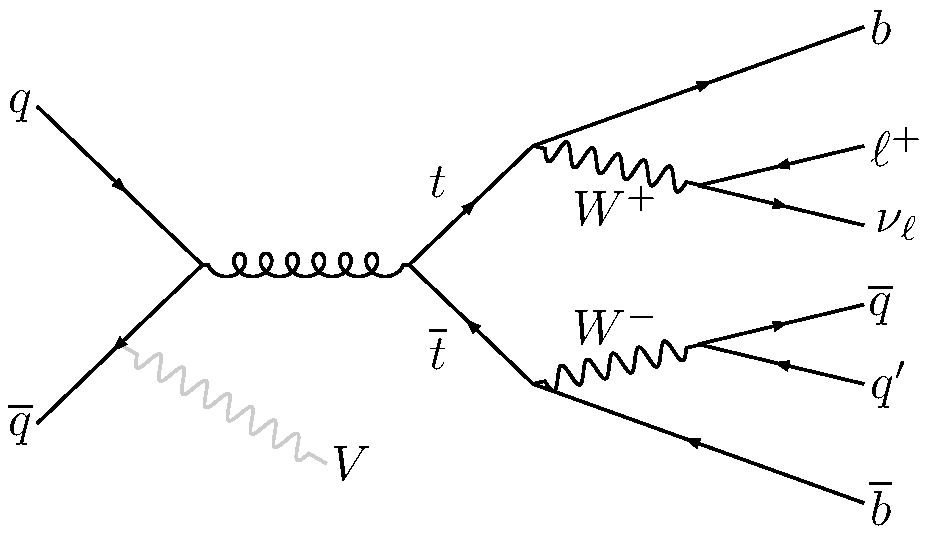
\includegraphics[width=0.4\textwidth]{fig/feynman/ttbar/ttV_onelep.pdf}\label{fig:ttV1l}}
    \caption{
        Lorem ipsum
    }
    \label{fig:single_t}
\end{figure}

\section{Event selection}
\subsection{Triggers}
\subsection{Signal region}
\subsection{Validation regions}

\section{Background estimation}

\section{Systematic uncertainties}

\section{Results}
\begin{figure}[htb]
    \centering
    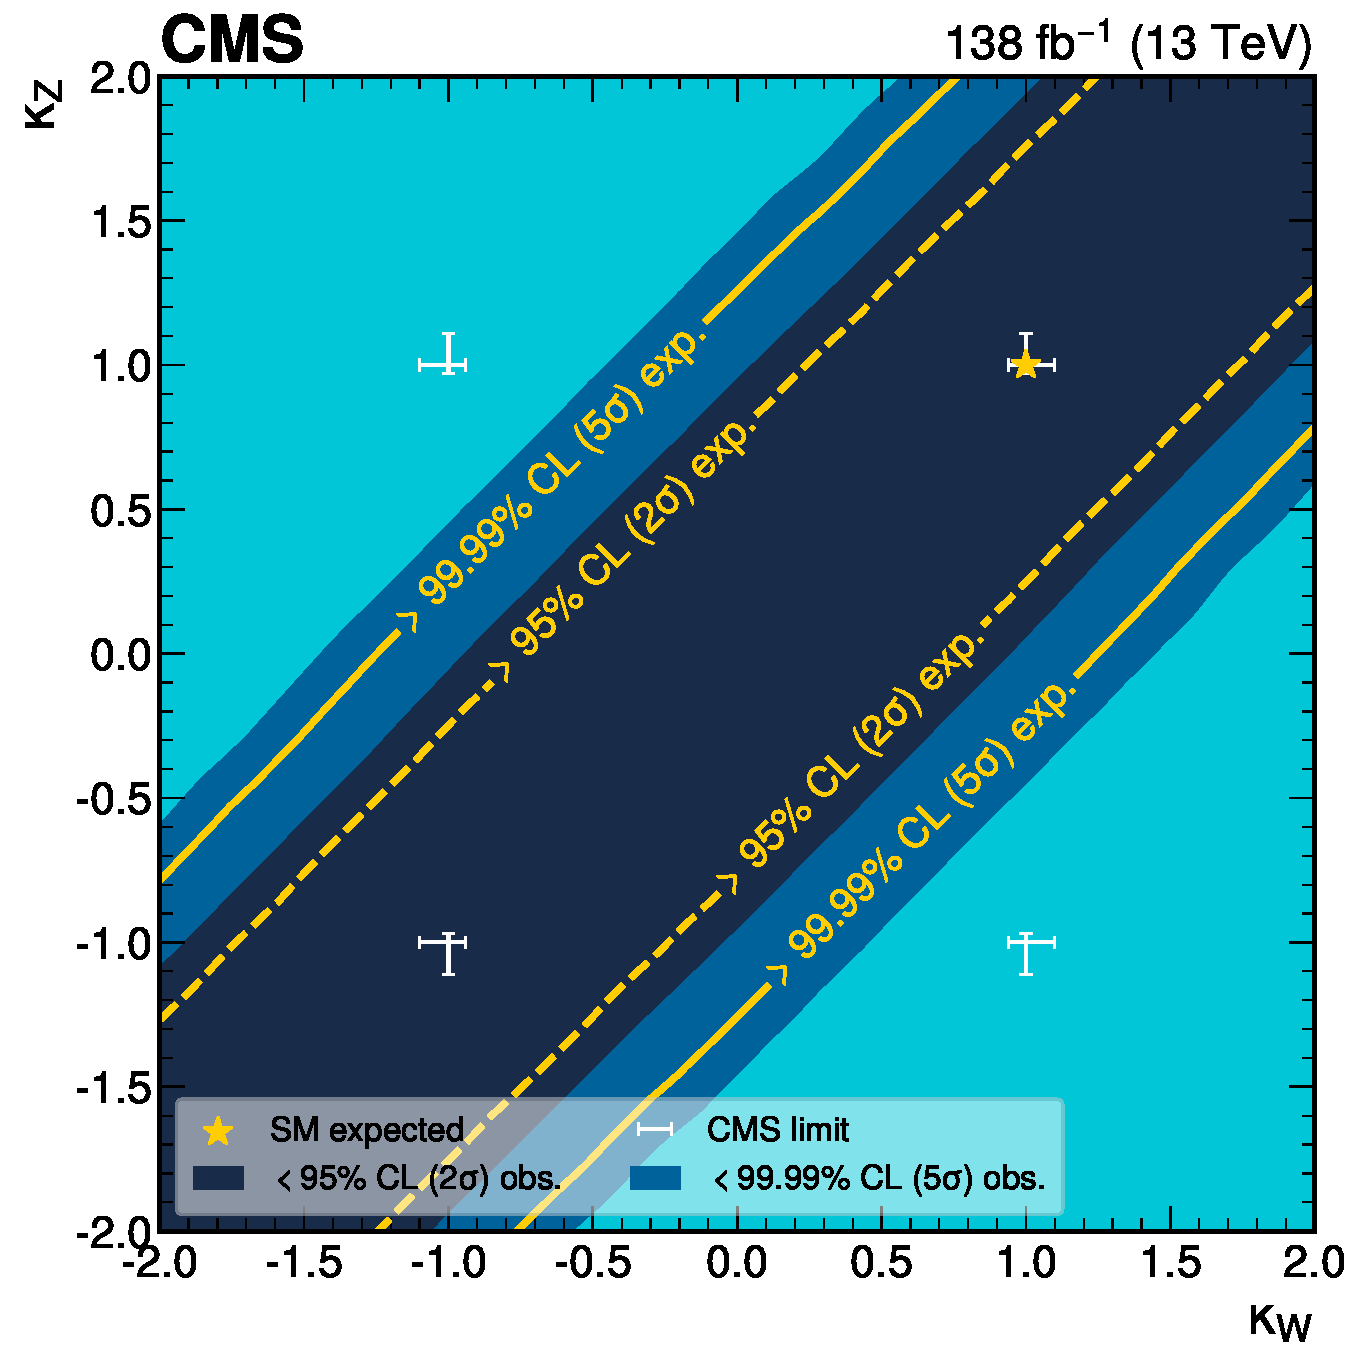
\includegraphics[width=0.5\textwidth]{fig/vbswh/exclusion_2D_contours_unblinded.pdf}
    \caption{
        Exclusion significance plotted as a function of \kW and \kZ.
        Opposite-sign scenarios ($\lambdaWZ < 0$) are excluded well beyond 5$\,\sigma$. 
    }
    \label{fig:vbswh_limit}
\end{figure}
